\documentclass[a4paper,14pt]{article}
\usepackage{float}
\usepackage{cite}
\usepackage[english,russian]{babel}
\usepackage{amssymb,amsmath,amsfonts}
\usepackage{color}
\usepackage{enumerate}
% \usepackage[dvips]{graphicx}
\usepackage{graphicx}
\usepackage{setspace}
\usepackage{xcolor}
\usepackage{fancyhdr}
\usepackage{tikz}

\textheight=220mm
\textwidth=160mm
\oddsidemargin=0.1in
\evensidemargin=0.1in

\title{sopromat}
\author{Даня Крутовский}
\date{October 2024}

\begin{document}

\pagestyle{fancy}
\fancyhead{}
\fancyhead[L]{\footnotesize{Современные проблемы математики и ее приложений}}
\fancyhead[R]{\footnotesize{Тезисы конференции}}
\fancyfoot{}
\fancyfoot[L]{\footnotesize{Екатеринбург, Россия}}
\fancyfoot[R]{\footnotesize{29 января -- 2 февраля и 16 февраля, 2023}}
\renewcommand{\footrulewidth}{0.1 mm}

\begin{center}
\textbf{Поиск оптимальной стратегии игры в симуляторе владельца продукта с помощью Deep RL}\\
\vspace{\baselineskip}
Крутовский Д.А.\\
\emph{Уральский федеральный университет, Екатеринбург, Россия}\\
krutovskiy.d@yandex.ru
\vspace{\baselineskip}\\

\end{center}
\vspace{\baselineskip}

\setcounter{equation}{0}
\setcounter{figure}{0}

\section{Введение}

\subsection{Что такое Reinforcement Learning?}

Обучение с подкреплением - это обучение тому, что надо делать, как следует отображать ситуацию в действия, чтобы максимизировать некоторый сигнал поощрения (вознаграждения), принимающий числовые значения \cite{Pi1}.

Агент - обучающийся и принимающий решение алгоритм.
Совокупность объектов вне агента, с которыми он взаимодействует, обозначается термином окружающая среда.
Между ними постоянно происходят взаимодействия: агент выбирает действия, окружающая среда реагирует, создает новую ситуацию и генерирует вознаграждение.

% Картинка
\begin{figure}[h]
    \centering
    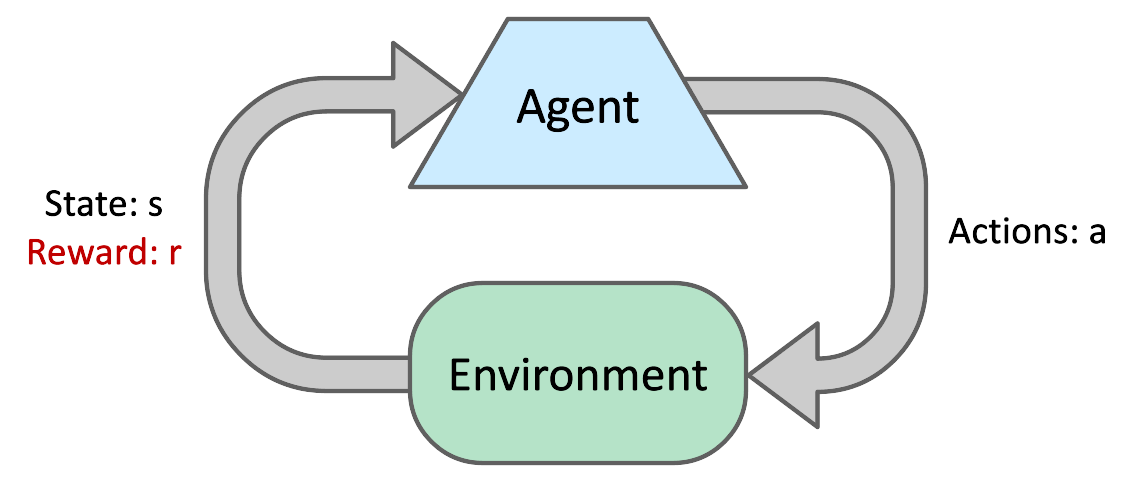
\includegraphics[width=0.5\linewidth]{images/reinforcement_learning_scheme.png}
    \caption{Иллюстрация обучения с подкреплением\cite{RL-Image}}
    \label{fig:rl_image}
\end{figure}

Более конкретно, на каждом дискретном шаге $t \in 1, 2, 3, ...$ агент получает описание состояния окружающей среды $s_t \in S$.
На основании этого описания агент выбирает действие $a_t \in A(s_t)$.
На следующем временном шаге агент получает вознаграждение $r_{t+1} \in \mathbb{R}$ и оказывается в новом состоянии $s_{t+1}$ \cite{Pi1}.

\subsection{О симуляторе владельца продукта}

В Product Owner Sim \cite{Pi2} вы начинаете с бюджетом 200 тысяч долларов и распоряжаетесь двумя роботами разработчиками.
Источником бюджета является долг, который составляет 300k, его нужно выплачивать по 9k за спринт.
Два разработчика тратят на задачи 20 часов за спринт, но каждый из них требует 10k, если нужно было работать.

Чтобы развивать продукт нужно проводить исследования или опросы пользователей.
Действие стоит денег, но создает задачи разных размеров.
Выпуск таких задач поднимает количество и лояльность пользователей.
От этих параметров зависит доходность продукта.

Для победы необходимо набрать 1M.

\section{Актуальность}

В разработке очень важную роль играет управление рабочими задачами в продукте.
Машинное обучение помогает человечеству автоматизировать и оптимизировать процессы.
Давайте попробуем автоматизировать управление продукта на упрощенной модели мира.
Для достижения цели взят DDQN - простой и эффективный алгоритм обучения с подкреплением, использующий глубокое обучение.

\section{Обзор существующих аналогов}

\subsection{Есть ли еще игры - симуляторы владения продукта?}

Game Dev Tycoon - игра, в которой вы создаете и развиваете свою собственную игровую компанию, начиная с 80-х годов.
В процессе создается множество игр. Сами игры описываются характеристиками тема, жанр, масштаб, технологии.

Software Inc. - симулятор разработки программного обеспечения, в котором вы создаете и управляете своей собственной IT-компанией. В этой игре очень высокий акцент на реализм.

\subsection{Есть ли алгоритмы, которые уже хорошо играют в пошаговые игры?}

Миру известны алгоритмы, которые обыгрывают человека в пошаговых играх - это AlphaGo,  она впервые выиграла у профессионального игрока в Го, поднявшись в турнире с самых слабых позиций.
После этого появилась AlphaGo Zero\cite{AlphaGo-Zero} - первая программа, победившая мирового чемпиона в игру Го.
Она обучалась с нуля, без каких либо подсказок или ограничейний от человека, в отличии от AlphaGo.
После появления версии Zero больших проектов для пошаговых игр не было.

Конкретно для Product Owner Simulator нет известных алгоритмов, которые обыгрывают человека.

\section{Описание процесса достижение цели}

Для успешного применения RL алгоритма к игре следует представить ее в виде среды с системой наград.
Среда должна иметь свойство марковости, то есть её поведение зависит только от текущего состояния и не зависит от предыдущих.

\subsection{Описание среды}

Рассмотрим среду с которой будет взаимодействовать агент.
Ее состояние можно описать набором числовых признаков, например, важно какой сейчас спринт, количество денег, лояльность пользователей и так далее.
Из исходного кода ясно, что состояние игры включает номер последнего спринта, в котором произошел релиз.
Эту информацию нельзя считать с экрана, но можно поддерживать самостоятельно.

Аккуратно собрав все данные, среда получает свойство марковости, что сильно упрощает процесс обучения агента.

В симуляторе владельца продукта конечное множество действий.
Например: начать спринт, приобрести работника или начать исследование.

% Где-то здесь можно привести скриншот из игры (или два)

Особой частью игры являются карточки задач.
Их количество постоянно меняется и это влияет на описание среды и доступные действия.
На практике, в один момент времени карточек в игре не очень много, поэтому было решено зафиксировать некоторое количество карточек и кодировать отсутствие карточки нулями.

В средах с конечным числом состояний и действий хорошо себя показывает Q обучением (Q-Learning)\cite{Pi3}, в котором строится таблица $S \times A$ и высчитывается ценность каждого действия в каждом состоянии.
После постороения таблицы агент может играть жадно, выбирая самые ценные ходы.
Мощность множества $S$ практически бесконечна, поэтому подход с таким алгоритмом не применим.

В данной среде присутствуют стохастические события, например, прирост пользователей благодаря релизу задачи или возникновения бага при релизе.

Среда имеет эпизодический характер, так как в ней можно победить - набрать 1M или проиграть - потратить весь бюджет или потерять всех пользователей.

\subsection{Агент}
Существует множество способов обучения агента в заданных условиях: Cross-Entropy, Monte-Carlo, SARSA, Deep Q-Learning.
Из перечисленных вариантов был выбран Deep Q-Learning\cite{DQN}, он хорошо показывает себя в бесконечных средах с конечным пространством действий.
Сходится быстрее перечисленных алгоритмов и обладает возможностью воспроизведения опыта (experience replay)\cite{Exp-Rep}.

На каждом шаге обучения метода Q-функция должна меняться следующим образом:

\[
Q(s_t, a_t) = Q(s_t, a_t) + \alpha 
    \left[
        r_{t+1} + \gamma \max_{a} Q(s_{t+1}, a) - Q(s_t, a_t) 
    \right].
\]

Для среды с бесконечным пространством состояний в основании алгоритма Q-Learning лежит нейронная сеть.
Она обрабатывает вектор параметров среды и выдает оценки суммарных наград для каждого действия.

В терминах функции ошибки для нейронной сети уравнение выше можно переписать так:

\[
Loss(\theta) = 
    \left(
        r_{t+1} + \gamma \max_{a} Q_(s_{t+1}, a; \theta^-) - Q(s_t, a_t; \theta) 
    \right) ^ 2.
\]

У DQN есть недостаток - излишняя оптимистичность.
Оценки алгоритма после обучения оказываются сильное выше, чем получаемые агентом награды.

Для решения этой проблемы предложена модификация алгоритма Double DQN\cite{DDQN}.
В ней добавляется еще одна нейросеть.
Она медленнее обучается, тем самым дольше остается пессимистичной.

%<!-- Модифицированная функция ошибки -->
\[
    Loss(\theta) = \left(
        r_{t+1} + \gamma Q(s_t, \argmax_{a} Q(s_t, a; \theta^-); \theta`)
        - Q(s_t, a_t; \theta)
    \right) ^ 2
\]

На практике оценки модифицированного алгоритма оказываются сильно ближе к полученным\cite{DDQN}.

% Можно сюда добавить графики сравнения алгоритмов

\subsection{Система наград}

В игре нет заранее заданной системы наград.
Ее нужно выбрать так, чтобы максимизация суммы наград за действия приближала агента к цели проекта.
Цель проекта обыгрывать человека в Симуляторе владельца продукта.
Обыграть человека значит подняться выше любого человека в лидерборде.
В лидерборде главным параметром является количество завершенных спринтов до победы.
Чем меньше спринтов тем, лучше.

Первая идея: штрафовать за каждый спринт.
За остальные действия не давать ни штрафа ни награды.

Результат: агент научился максимально быстро проигрывать. Это произошло, потому что для проигрыша достаточно 5-7 спринтов, а для победы более 45. И из-за того, что выиграть достаточно сложно, штраф за проигрыш превращается в константную награду, на которую агент не может повлиять.

% Как нибудь показать это

Вторая идея: награждать за валидные действия и сильно награждать за победу.
В этом случае коэффициент дисконтирования мотивировал играть быстрее.

Результат: агент научился дольше играть.
В частности достигать спринта, в котором заканчивается выплата кредита.
После выплаты кредита в игре появляются карточки багов и тех. долга, которые усложняют процесс игры.

Чтобы DDQN обучался на однородных данных, было решено разделить игру на этапы.
Первый этап - обучение, в котором нужно исследовать, декомпозировать и выпустить одну задачу.
На этом этапе действия тривиальны и агент без труда учится проходить обучение за минимальное количество спринтов.

Второй этап - самый сложный, выплата кредита.
В нем нужно довести до релиза множество задач, постепенно накапливая количество пользователей и их лояльность.
На этом этапе агент ограничен по количеству спринтов и должен максимизировать набор параметров, такие как благосостояние и удовлетворенность пользователей.

Третий этап - набор необходимого капитала.
После выплаты кредита, денег за спринт становится больше, но игра становится сложнее.

Оказалось, что при достаточно хорошей игре во втором этапе, накопленных денег и пользователей достаточно, чтобы делать пустые спринты, то есть не выполнять никакой работы.
Таким образом количество пользователей убывает с каждым спринтом, но даже так дохода достаточно, чтобы накопить миллион.

\subsubsection{Подсказки валидных действий}

В игре доступные действия определяются её состоянием.
Например, исследование, которое создает карточку, стоит \$80k.
Если сейчас денег меньше, то провести исследование нельзя.
Алгоритму это может подсказать среда.
После применения действия среда не меняется, а награда за действие будет отрицательной.
Чтобы учитывать недоступные действия агент должен выучить закономерности и зависимости действий от среды.

Гипотеза: если агент будет выбирать только из доступных действий, обучение ускорится и достигнет качественно лучшего результата.
Эксперимент поставлен так: обучаться агент будет на первых 35 спринтах.
Если игра не закончена, доигрывание будет пустыми спринтами.
Результат: агент научился выигрывать с определенным шансом.

На графике ниже изображен усредненный процесс обучения агентов.
Оранжевым изображен агент, который не получал подсказки о доступных действиях.
Синим - агент, который выбирал действия только из доступных.

\begin{figure}[h]
    \centering
    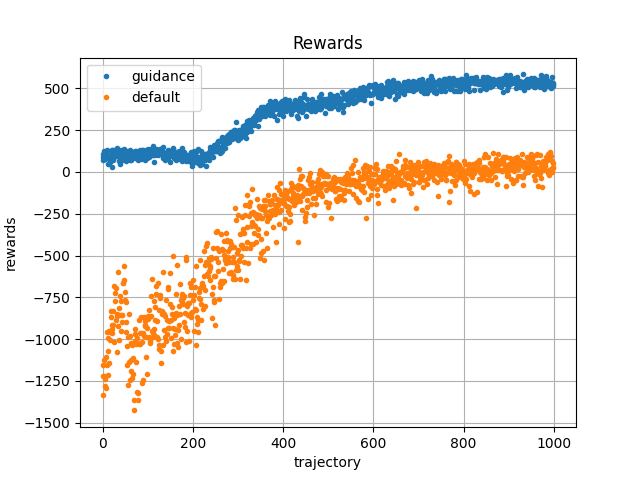
\includegraphics[width=0.5\linewidth]{images/guidance_rewards.png}
    \caption{Суммарные награды агентов}
    \label{fig:guidance-exp}
\end{figure}

Модификация алгоритма позволила побеждать в игре с 13\% вероятностью. До этого агент не мог победить в игре.

\subsubsection{Модификация системы наград}

Гипотеза: если агента больше награждать за потенциал, который можно потратить жадным доигрыванием, агент накопит больше капитала к 35-му спринту.
Таким образом шанс выиграть после работы агента станет сильно выше.
Результат: получилось увеличить вероятность победы и не увеличить победный спринт.

Из-за увеличения размера сети процент побед агента с обычной системой наград поднялся до 27\%. А процент побед для новой системы наград оказался 47\%.

% Тут хорошо подойдет табличка и p-values

\subsection{Лидерборд}
Для достижения цели проекта нужно добиться того, чтобы обученный агент попал в лидерборд.
Для попадания в лидерборд агент должен совершать действия в веб версии игры.
Автоматизировать работу с браузером позволяет библиотека Selenium\cite{Selenium}.
После загрузки страницы появляется задача считывания состояния игры, чтобы агент смог выбрать оптимальное действие.
По техническим причинам в браузере игра описывается только картинкой.
Для работы с изображениями подойдет OpenCV\cite{OpenCV} - это мощный инструмент компьютерного зрения.
В фиксированных местах расположены необходимые данные, такие как номер спринта, текущий капитал и так далее.
Поэтому считывание цифр с помощью сравнения с шаблоном - самый простой и подходящий вариант.

После считывания состояния, передачи его агенту, появляется действие, которое нужно совершить.
Обычно это несколько кликов по экрану.

\section{Оценка и сравнение результатов}

До лидерборда алгоритм еще не добрался.
Агент обучается на логике игры, переписанной с Godot на Python.
Эта логика перенесена с использованием оригинального кода.

При валидации алгоритма - шанс выиграть в игре составляет 68 процентов.
При этом минимальный выигрышный спринт - 47.
Это ровно первое место в текущем лидерборде.

Не очень большая нейронная сеть может играть на уровне человека в симулятор владельца продукта!

\section{Выводы и возможные направления дальнейших действий}

Для улучшений результатов алгоритма можно попробовать увеличить размер нейронной сети лежащей в основе алгоритма.
Или же попробовать применить более сложные алгоритмы RL.

Можно развить симулятор владельца продукта, немного приблизив его к реальности.
И с помощью текущих наработок адаптировать ИИ побеждать в следующий версии игры.
Возможно, таким итеративным образом можно достичь уровень ИИ способного быть владельцем настоящего продукта.

\small
\begin{thebibliography}{99}

\bibitem{Pi1}
Р.~С.~Саттон, Э.~Г.~Барто. Обучение с подкреплением. {\it Адаптивные и интеллектуальные системы}, (2014), 12--13, 74--75

\bibitem{RL-Image}
UC Berkeley CS188 Intro to AI -- Course Materials
https://ai.berkeley.edu/lecture\_slides.html

\bibitem{Pi2} Игра Симулятор владельца продукта 
https://npg-team.itch.io/product-owner-simulator

\bibitem{AlphaGo-Zero}
D.~Silver, J.~Schrittwieser, K.~Simonyan, et al. Mastering the game of Go without human knowledge. Nature 550, 354–359 (2017). https://doi.org/10.1038/nature24270

\bibitem{Pi3}
C.~J.~C.~H.~Watkins, P.~Dayan Q-learning. Mach Learn 8, 279–292 (1992). https://doi.org/10.1007/BF00992698

\bibitem{DQN}
V.~Mnih, K.~Kavukcuoglu, D.~Silver, A.~Graves, I.~Antonoglou, D.~Wierstra, M.~ Riedmiller
Playing Atari with Deep Reinforcement Learning
arXiv:1312.5602

\bibitem{Exp-Rep}
Lin, L.-J. Self-improving reactive agents based on reinforcement learning, planning and teaching. Machine learning,
8(3-4):293–321, 1992.

\bibitem{DDQN}
H.~van Hasselt, A.~Guez, D.~Silver
Deep Reinforcement Learning with Double Q-learning
https://arxiv.org/abs/1509.06461

\bibitem{Selenium}
https://www.selenium.dev/

\bibitem{OpenCV}
https://opencv.org/

\end{thebibliography}

\normalsize

\end{document}
